\documentclass[a4paper]{article}
\usepackage{cmap}
\usepackage[utf8]{inputenc}
\usepackage[T2A]{fontenc}
\usepackage{amsfonts}
\usepackage{amsmath, amsthm}
\usepackage{amssymb}
\usepackage{hyperref}
\usepackage{multicol}
\usepackage{xcolor}
\usepackage{graphicx}
\usepackage{wrapfig}

\newcommand\letsymbol{\mathord{\sqsupset}}
\usepackage[russian]{babel}
\renewcommand\qedsymbol{$\blacktriangleright$}
\newtheorem{theorem}{Теорема}[section]
\newtheorem{lemma}{Лемма}[section]
\theoremstyle{definition}
\newtheorem*{example}{Пример}
\newtheorem*{definition}{Определение}
\newtheorem*{statement}{Утверждение}
\theoremstyle{remark}
\newtheorem*{remark}{Замечание}

\setlength{\topmargin}{-0.5in}
\setlength{\oddsidemargin}{-0.5in}
\textwidth 185mm
\textheight 250mm

\begin{document}
\tableofcontents
\section{Введение}
\begin{definition}[Методы оптимизации]
    Раздел прикладной математики, содержание которого составляет теория и методы решения оптимизационных задач
\end{definition}
\begin{definition}[Оптимизационная задача]
    Задача выбора наилучшего варианта (в некотором смысле) из имеющихся
\end{definition}
\begin{definition}[Задача оптимизации]
        $\begin{cases}
        f(x)\to \min(\max) \\
        x\in D
    \end{cases}$
\end{definition}
D - множество допустимых решений, $f:D\to \mathbb{R}$
\begin{definition}[Задача МП]
    $\begin{cases}
        (1) f(x)\to \min (\max) [extr] (opt)\\
        (2) g_i(x) \# 0, i=1,\dots, m - \text{ограничения} \\
        (3)x\in \mathbb{R}^n 
    \end{cases}$
    \(x = (x_1, ..., x_n) \, f(x): \mathbb{R}^n \to \mathbb{R}, \, g_i(x) : \mathbb{R}^n \to \mathbb{R}\)
\end{definition}
\begin{definition}[Допустимое решение]
    $x\in \mathbb{R}^n$, удовл (2), называется допустимым решением задачи.
\end{definition}
\begin{definition}[Оптимальное решение]
    Допустимое решение $x^*\in D$ задачи 1 - 3 называется оптимальным решением, если $f(x) \leq f(x^*) \, \forall x\in D$ в случае задачи максимизации и $f(x) \geq f(x^*) \, \forall x\in D$ в случае задачи минимизации
\end{definition}
Глобальный оптимум -  $x^*$
\begin{definition}[Локальный оптимум]
    Допустимое решение $\widetilde{x}\in D$ задачи 1 - 3 называется локальным оптимумом, если $f(x) \leq f(\widetilde{x})$ для всех х из некоторой окрестности $\widetilde{x}$ в случае задачи максимизации и $f(x) \geq f(\widetilde{x})$ для всех х из некоторой окрестности $\widetilde{x}$ в случае задачи минимизации
\end{definition}
\begin{definition}[Разрешимая/неразрешимая]
    Задача 1 - 3, которая обладает оптимальным решением, называется разрешимой, иначе неразрешимой
\end{definition}
\section{Линейное программирование}
\subsection{Постановка задачи (ЛП), теоремы эквивалентности}
\begin{definition}[Общая задача ЛП]
$    \begin{cases}
        f(x) = c_0 + \sum_{j = 1}^n c_j x_j \to \max (\min) \\ 
        \sum_{j = 1}^{n} a_{ij}x_j \# b_i, \, i = 1, \dots, m \\
        x_j \geq 0, j \in J\subseteq \{1, \dots, n\}
    \end{cases}$, где \(x = (x_1, ..., x_n)\in \mathbb{R}^n\) -  вектор переменных

    Матричная запись:

    $\begin{cases}
        f(x) = (c, x) \to \max(\min)\\
        Ax \# b \\
        x_j \geq 0, j \in J\subseteq \{1, \dots, n\}
    \end{cases}$, $x = \begin{pmatrix}
        x_1 \\ \vdots \\ x_n
        \end{pmatrix}, b = \begin{pmatrix}
            b_1 \\ \vdots \\ b_m
            \end{pmatrix}, 
            A = \begin{pmatrix} 
                a_{11} & \dots  & a_{1n}\\
    \vdots & \ddots & \vdots\\
    a_{m1} & \dots  & a_{mn} 
    \end{pmatrix}$
\end{definition}
\begin{definition}[Стандартная (симметрическая) форма]
    $\begin{cases}
        f(x) = c_0 + \sum_{j = 1}^n c_j x_j \to \max \\
        \sum_{j = 1}^{n} a_{ij}x_j \leq b_i, \, i = 1, \dots, m \\ 
        x_j \geq 0, j = 1, \dots, n
    \end{cases}$
\end{definition}
\begin{definition}[КЗЛП]
    $\begin{cases}
        f(x) = c_0 + \sum_{j = 1}^n c_j x_j \to \max\\
        \sum_{j = 1}^{n} a_{ij}x_j =b_i, \, i = 1, \dots, m \\ 
        x_j \geq 0, j = 1, \dots, n
    \end{cases}$
\end{definition}
\begin{definition}[Основная задача ЛП]
    $\begin{cases}
        f(x) = c_0 + \sum_{j = 1}^n c_j x_j \to \max\\
        \sum_{j = 1}^{n} a_{ij}x_j \leq b_i, \, i = 1, \dots, m
    \end{cases}$
\end{definition}
\begin{definition}[Эквивалентные ЗЛП (ЗМП)]
    Две задачи ЛП $P_1, P_2$ называются \textit{эквивалентными}, если любому допустимому решению задачи $P_1$ соответствует некоторое допустимое решение задачи $P_2$ и наоборот, причем оптимальному решению одной задачи соответствует оптимальное решение другой задачи.
\end{definition}
\begin{theorem}[Первая теорема эквивалентности]
    Для любой ЗЛП существует эквивалентная ей каноническая ЗЛП.
\end{theorem}
\begin{theorem}[Вторая теорема эквивалентности]
    Для любой ЗЛП существует эквивалентная ей симметрическая ЗЛП.
\end{theorem}
\subsection{Каноническая задача ЗЛП. Базисные решения}
\begin{definition}[Базисное решение]
    Пусть $\overline{x}$ - решение $Ax = B$. Тогда вектор $\overline{x}$ называется базисным решением СЛАУ, если система вектор-столбцов матрицы А, соответствующая ненулевым компонентам вектора $\overline{x}$, ЛНЗ
\end{definition}
\begin{remark}
    Если система однородная, то x = $\overline{0}$ - базисное решение
\end{remark}
\begin{definition}
    Неотрицательное базисное решение СЛУ называется базисным решением канонической задачи ЛП
\end{definition}
\begin{definition}[Вырожденное БР]
    $\overline{x}$ - БР КЗЛП называется вырожденным, если число ненулевых компонент меньше ранга матрицы А, иначе невырожденное
\end{definition}
\begin{lemma}
    Если x и x' - Б.Р. КЗЛП, $x\neq x'$, то \[J(x) \neq J(x'), J(x)\subset J(x'), J(x) \supset J(x'),\] где $J(x) = \{j | x_j \neq 0, j = 1\dots n\}$
\end{lemma}
\begin{theorem}[О конечности множества базисных решений]
    Число базисных решений КЗЛП конечно
\end{theorem}
\begin{theorem}[О существовании оптимальных БР]
    Если КЗЛП разрешима, то существует ее оптимальное БР
\end{theorem}
\subsection{Симплекс-метод}
Рассмотрим КЗЛП.
\subsubsection{Симплекс-метод для приведенной ЗЛП}
\begin{definition}[Система с базисом]
    СЛАУ - СЛАУ с базисом, если в каждом уравнении имеется переменная с коэффициентом +1, отсутствующая в других уравнениях. Такие переменные будем называть базисными, остальные не базисными
\end{definition}
\begin{definition}[ПЗЛП]
    КЗЛП называется приведенной, если 
    \begin{enumerate}
        \item СЛАУ $Ax = B$ является системой с базисом
        \item Целевая функция выражена через небазисные переменные
    \end{enumerate}
\end{definition}
\begin{definition}[Прямо допустимая симплексная таблица]
    СТ называется прямо допустимой, если $a_{i0}\geq 0, i = 1, \dots, m$ (bшки)
\end{definition}
\begin{definition}[Двойственно допустимая симплексная таблица]
    СТ называется двойственно допустимой, если $a_{0j}\geq 0, i = 1, \dots, n+m$ (cшки)
\end{definition}
\begin{theorem}
    Если симплекс-таблица является прямо допустимой и $a_{0j}\geq 0, j = 1\dots, n+m$, то соответствующее базисное решение является оптимальным 
\end{theorem}
\begin{theorem}
    Если в симплекс-таблице существует $a_{0q}< 0, a_{iq}\leq 0, \, \forall i = 1\dots, m$, то задача неразрешима, потому что f неограничена на множестве допустимых решений
\end{theorem}
\begin{theorem}
    Если ведущая строка выбирается из условия минимума ключевого отношения, то следующаяя симплексная таблица будет прямо допустимой
\end{theorem}
\begin{theorem}[Об улучшении базисного решения]
    Если $\exists a_{0j}< 0, j = 1\dots n+m$, то возможен переход к новой прямо допустимой симплекс таблице, причем $f(x)\leq f(x')$, где x - БР старой таблицы, x'- БР новой таблицы,
    f(x) = $a_{00}$ старой таблицы, f(x') = $a_{00}-\frac{a_{p0}a_{0q}}{a{pq}}, a_{p0} = 0$ - вырожденное решение
\end{theorem}
\subsection{Каноническая ЗЛП}
\paragraph*{Метод искусственного базиса}
\begin{definition}[искусственные]
    $t_i\geq 0$ - искусственные переменные
\end{definition}
\begin{remark}[Свойства ВЗЛП]
    \begin{enumerate}
        \item ВЗЛП почти приведенная (нужно выразить $t_i$)
        \item $h(x, t) \leq 0 \quad \forall (x, t)\in \widetilde{D}$
        \item $\widetilde{D}\neq 0$ (например, есть $(0, \dots, n, b_1, \dots, b_m)$, n нулей)
        \item ВЗЛП всегда разрешима 
    \end{enumerate}
\end{remark}
\begin{theorem}[О существовании допустимого решения исходной КЗЛП]
    $$D\neq 0 \Leftrightarrow h^*(x, t)=0$$
\end{theorem}
\begin{theorem}[О преобразовании КЗЛП в эквивалентную ей приведенную]
    Если множество допустимых решений исходной КЗЛП непусто, то ПЗЛП, эквивалентная исходной КЗЛП, может быть получена из последней симплекс таблицы - таблицы ВЗЛП
\end{theorem}
\subsection{Двойственность в ЛП}
\begin{definition}
    Будем говорить, что знаки линейных ограничений ЗЛП согласованы с целевой функцией, если в задаче на max ограничения неравенства имеют вид "$\leq$", а в задаче на min ограничения на неравенство имеют вид "$\geq$"
\end{definition}
\begin{definition}[Двойственная задача]
    Для ЗЛП I двойственной задачей II является ЗЛП вида:
    $$f(x) = \sum_{j = 1}^n c_j x_j \to \max \leftrightarrow g(y) = \sum_{i = 1}^m b_i y_i\to \min,$$
    $$\sum_{j = 1}^n a_{ij} x_j \leq b_i, i = 1, \dots, l \leftrightarrow y_i\geq 0, i = 1...l,$$
    $$\sum_{j = 1}^n a_{ij} x_j = b_i, i = l+1, \dots m \leftrightarrow y_i\in \mathbb{R}, i = l+1, \dots, m,$$
    $$x_j\geq 0, i = 1, \dots p\leftrightarrow \sum_{i = 1}^m a_{ij} y_i \geq c_j, j = 1, \dots, p$$
    $$x_j \in \mathbb{R}, j = p+1, \dots n \leftrightarrow \sum_{i = 1}^m a_{ij} y_i = c_j, j = p+1, \dots, n$$
        Задачу I называют прямой, а II - двойственной. Стрелки соответствуют сопряженным ограничениям
\end{definition}
\begin{theorem}[Основное неравенство двойственности]
    $$\forall x\in D_I, \forall y\in D_{II}, f(x)\leq g(y)$$
\end{theorem}
\subsection{Теоремы двойственности}
\begin{lemma}[основная лемма]
    Пусть $\forall x\in D_I \neq \varnothing, f(x)\leq M < +\infty\implies \exists y \in D_{II}\, g(y)\leq M$
\end{lemma}
\begin{theorem}[Первая теорема двойственности]
    Если одна из пары двойственных задач разрешима, то разрешима и другая, причем оптимальное значение целевых функций совпадает, т.е $f(x^*) = g(y^*)$, где $x^*, y^*$ - оптимальные решения задач I, II соответственно
\end{theorem}
\begin{theorem}
    Вектор $x^* \in D_I$ является оптимальным решением задачи 
    I $\Leftrightarrow \exists y^* \in D_{II}$ т.ч  $g(y^*) = f(x^*)$    
\end{theorem}
\begin{definition}[Условия дополняющей нежесткости]
    Будем говорить, что $x\in D_I, y \in D_{II}$ удовлетворяют УДН, если при подстановке в любую пару сопряженных неравенств хотя бы одно из них обращается в равенство. Это означает, что следующие характеристические произведения обращаются в 0:
    \[(\sum_{j = 1}^n a_{ij}x_j - b_i)y_i = 0, i  = 1, \dots m\]
    \[x_i (\sum_{i = 1}^m a_{ij}y_i - c_j) = 0, j = 1, \dots n\]
\end{definition}
\begin{theorem}[Вторая теорема двойственности]
    $x^* \in D_I, y^*\in D_{II}.$ оптимальны в задачах I, II тогда и только тогда, когда они удовлетворяют УДН.
\end{theorem}
\begin{theorem}[Второй критерий оптимальности (следствие)]
    \(x^* \in D_I\) является оптимальным решением I \(\Leftrightarrow\)
    \(\exists y^* \in D_{II}\) т.ч. \(x^*\) и \(y^*\) удовлетворяют УДН
\end{theorem}
\subsection{Критерий разрешимости ЛП}
\begin{definition}[Точная верхняя грань функции]
    $M^*$ называется точной верхней гранью функции f(x) на множестве D, если \begin{enumerate}
        \item $\forall x \in D \quad f(x) \leq M^*$
        \item $\forall M < M^* \quad \exists x\in D \quad f(x)> M$
    \end{enumerate}
\end{definition}
\begin{lemma}[О точной верхней грани функции g(y) на $D_{II}$]
    $M^*< +\infty$ - точная верхняя грань $f(x)$ на $D_{I}$, тогда $\forall y \in D_{II} \quad g(y) \geq M^*$
\end{lemma}
\begin{theorem}[Критерий разрешимости]
    Целевая функция задачи ЛП ограничена сверху (снизу) на непустом множестве допустимых решений тогда и только тогда, когда задача максимизации (минимизации) разрешима
\end{theorem}
\subsection{Классификация пар двойственных задач}
\begin{theorem}[Малая теорема двойственности]
    Если $D_I \neq \varnothing, D_{II} \neq \varnothing\implies$ обе задачи точно разрешимы
\end{theorem}
\begin{theorem}[О причинах неразрешимости ЗЛП]
    $D_{I}\neq \varnothing$, целевая функция неограничена сверху на $D_I$ тогда и только тогда, когда II неразрешима, так как $D_{II}=\varnothing$
\end{theorem}
\paragraph*{Классификация}
\begin{enumerate}
    \item $D_I\neq \varnothing, D_{II} \neq \varnothing$ обе задачи разрешимы, т.к $f(x^*) = g(y^*)$
    \item $D_I\neq \varnothing, D_{II} = \varnothing$ обе неразрешимы, т.к $f(x)$ неограничена, $D_{II}=\varnothing$
    \item $D_I = \varnothing, D_{II} \neq \varnothing$ обе неразрешимы, т.к  $D_I = \varnothing, g\to +\infty$ на $D_{II}$
    \item $D_I = \varnothing, D_{II} = \varnothing$ обе неразрешимы
\end{enumerate}
\subsection{Экономическая интерпретация двойственной задачи и теорема двойственности}

\paragraph*{Экономический смысл двойственной переменной и задачи}
Линейные ограничения двойственной задачи связывают задачи всех ресурсов,
идущих на производство 1 ед. продукции, с прибылью от продажи этой единицы продукции $\implies y_i$ измеряются в ед. стоимости

Т.к $y_i$ соответствует ресурсам, то $y_i$ - некая цена ресурса. Будем называть ее условной ценой (двойственной оценкой на ресурсы).

Для интерпретации двойственной задачи посмотрим на предприятие как \textbf{на продавца ресурсов.}

Задача (II) определяет справедливые цены на ресурсы, в которой требуется определить набор оценок всех ресурсов, при котором для каждого вида продукции ресурсов затрачено на производство 1 ед. продукции \textbf{не меньше} дохода от ее реализации, при этом суммарная оценка ресурсов будет минимальна

\begin{theorem}[1]
    Суммарная прибыль от продажи произведенной продукции =  суммарной оценке всех ресурсов
\end{theorem}
$y_i^*$ - ценность i-того ресурса для производителя - доход, который может быть получен от 1 единицы использованного i-того ресурса
\begin{theorem}[2]
    \begin{itemize}
        \item ресурс 1 и 2 расходуется полностью - их называют дефицитными - они соответствуют $y_i^*\ge 0$

        % ресурс 3 расходуется не полностью 
        \item $x_1^* > 0, x_2^* > 0$, т.е продукция произвед. $\implies$ расходы ресурсов равны стоимости продажи этих продуктов

        если стоимость ресурсов, требуемых для производства 1 ед. прод > прибыль
    \end{itemize}
\end{theorem}
\subsection{Анализ на чувствительность модели ЛП}
\begin{definition}[Анализ чувствительности модели ЛП]
    Анализ чувствительности модели ЛП - исследование влияния изменения входных данных на оптимальное решение
\end{definition}
Рассмотрим частную задачу - анализ изменения оптимального решения при изменении запаса только одного ресурса.

$y_i^*$ рассмотрим как потенциальную возможность получить доп. доход.

Рассмотрим три задачи:

\[\begin{cases} (I)f = (c, x) \to \max \\ Ax\le b \\ x\ge 0 \\ b = (b_1, \dots, b_m) \end{cases}\]
\[\begin{cases} (I')f = (c, x) \to \max \\ Ax\le b' \\ x\ge 0 \\ b' = (b_1+\Delta b_1, \dots, b_m), D_I \subset I' \end{cases}\]
\[\begin{cases} (\overline{I})f = (c, x) \to \max \\ Ax\le \overline{b} \\ x\ge 0 \\ \overline{b} = \alpha b + (1- \alpha )b', \alpha \in (0, 1) \end{cases}\]

\begin{definition}[решения, имеющие одинаковую структуру]
    Будем говорить, что решения $x\in D_I$ и $x' \in D_{I'}$ имеют одинаковую структуру, если
    \begin{enumerate}
        \item совпадают по ассортименту, т.е. $x_j = 0 \Leftrightarrow {x_j}' = 0 j = 1, \dots, n$
        \item имеют одни и те же дефицитные ресурсы, т.е i-тое ограничение I выполняется на равенство тогда и только тогда, когда i-тое ограничение I' задачи выполняется на равенство
    \end{enumerate}
\end{definition}
\begin{lemma}[О планах одинаковой структуры]
    Пусть x* - опт решение I и $x' \in D_I'$ - решение той же структуры, тогда
    \begin{enumerate}
        \item x' - опт решение задачи I';
        \item для любого $\alpha \in (0, 1)$ существует оптимальное решение $\overline{I}$ имеющее эту же структуру
    \end{enumerate} 
\end{lemma}
\begin{remark}
    Изменять запас ресурса $P_1$ можно до тех пор, пока в задаче I' будет существовать оптимальный план той же структуры, что и в I
\end{remark}
\begin{definition}[Малое (допустимое) изменение]
    Малое (допустимое) изменение ресурса P1 - такое изменение $\Delta b_1 = b_1' - b_1$ для кот в задаче I' существует оптимальное решение той же структуры, что и оптимальное решение исходной задачи I
\end{definition}
В силу леммы, если $\Delta b_1$ - допустимое изменение ресурса, то и все меньшие изменения также допустимы.

Пусть $F(b_1, \dots, b_m)$ - max доход, который можно получить при запасах ресурсов $b_i$

\begin{definition}[3-я теорема двойственности]
    При допустимом изменении i-того ресурса приращение целевой функции прямо пропорционально изменению ресурса с коэффициентом пропорциональности, равным $y_i^*$

    $$\Delta_i F = \Delta b_i y_i^*, \Delta_i F = F(b_1, \dots, b_{i-1}, b_i + \Delta b_i, \dots, b_m)-F(b_1, \dots, b_{i-1}, b_i, \dots, b_m)$$
\end{definition}
\subsection{О конечности симплекс-метода}
\begin{definition}[вырожденная КЗЛП]
    КЗЛП является вырожденной, если среди ее БР имеются вырожденные.
\end{definition}
\begin{enumerate}
    \item Если КЗЛП не является вырожденной - в процессе работы симплекс-метода $f(x_1) < \dots < f(x^*)$ (с-метод конечен)
    \item $a_{p0} = 0\implies f(x) = f(x')$ БР сохраняется, но меняется набор базисных переменных 
\end{enumerate}
после некоторого числа итераций возможен возврат к уже встречавшимся ранее наборам базисных переменных - с-м может зациклиться
\paragraph*{Уточняющие правила}
\begin{enumerate}
    \item Правило Данцига - выбирается столбец $$a_{0q} = \min_{j: a_{0j}< 0} a_{0j}$$
    \item правило наибольшего приращения: выбираем такое q, при котором приращение наибольшее
    $$a_{00}' = a_{00} - \frac{a_{0q} a_{p0}}{a_{pq}}$$
    \item Правило Бленда

    Cтрока и столбец выбираются в соответствии с обычными правилами выбора, причем каждый раз из возможных выбирается переменная с наименьшим номером
    \item Лексикографическое правило выбора ведущей строки
    $$\frac{\overrightarrow{a_p} }{a_{pq}}  = \min_{a_{iq}>0}\frac{\overrightarrow{a_i} }{a_{iq}}$$
\end{enumerate}
\subsection{Двойственный симплекс-метод}
$$\textsubscript{мне по. чисто по.}$$
\section{Целочисленное линейное программирование}
\subsection{Задачи ЦЛП}
\begin{definition}[Задача ЦЛП]
        \begin{equation}
            f(x) = \sum_{j=1}^n c_j x_j \to \max
        \end{equation}
     \begin{equation}
        \sum_{j = 1}^n a_{ij}x_j \# b_i, i = 1, \dots, m 
     \end{equation}
    \begin{equation}
        x_j \ge 0, j = 1, \dots, n
    \end{equation}
     \begin{equation}
        x_j \in \mathbb{Z}, j =1, \dots, n 
     \end{equation}
    
    \(c_j, b_i, a_{ij} \in \mathbb{Z} \text{ или } \mathbb{Q}\)
\end{definition}
\begin{definition}[Релаксационная задача]
    (1-3) - задача ЛП, которая называется соответствующей непрерывной или релаксационной задачей.
\end{definition}
$D$ - область допустимых решений (1 - 3), а $D_Z$ - множество всех целочисленных
точек области D.
\subsection{Метод отсечения}
\begin{enumerate}
    \item [шаг 1] Решается задача ЛП (1-3). Если она не имеет решения, то и задача ЦЛП не имеет решения. \textbf{СТОП}
    \item [шаг 2] Пусть $x^0\in D$ - оптимальное решение задачи ЛП. Если оно из $D_Z$ - то оно оптимальное решение задачи ЦЛП. \textbf{СТОП}
    \item [шаг 3] Строится дополнительно линейное ограничение (отсечение)
    \[\sum_{j = 1}^n \alpha_j x_j \ge \beta\]
    Отсечение добавляется к задаче ЛП.
    После этого осуществляется возврат на шаг 1, на котором решается задача ЛП.
\end{enumerate}
\begin{definition}[Правильное отсечение]
    Доп. ограничение - правильное, если
    \begin{enumerate}
        \item оно отсекает часть области D, содержащее нецелочисленное оптимальное решение $x^0$ текущей задачи ЛП.
        \item В отсекаемой части области не должно быть ни одного допустимого решения задачи ЦЛП (ограничение сохраняет все допустимые целочисленные решения)
    \end{enumerate}
\end{definition}
\begin{enumerate}
    \item $\sum_{j = 1}^n \alpha_j x_j^0 < \beta$
    \item  $\sum_{j = 1}^n \alpha_j x_j \ge \beta \quad \forall x \in D_Z$
\end{enumerate}
\subparagraph*{Отсечение Гомори}
Имеем оптимальную с-таблицу $a_{ij, i = 0, \dots, m, j = 0, \dots, n}$

Рассмотрим $a_{l0}\notin \mathbb{Z}$. l выбираем с наибольшей дробной частью по правилу "первая сверху" ($l\in \{0, \dots, n\}$)

Дробная часть: $\{\frac54\} = \frac14$, $\{-\frac54\} = \frac34$

Дополнительное ограничение:
\[\sum_{j\in Nb} \{a_{lj}\}x_j \geq \{a_{l0}\}\]
Приводится к канон. виду и добавляется в ограничение
\begin{theorem}
    Отсечение Гомори является правильным.
\end{theorem}
\subparagraph*{Первый алгоритм Гомори}
\begin{enumerate}
    \item Все ЗЛП решаются ЛДСМ (кроме, быть может, самой первой)
    \item Специальное правило выбора производящей строки - "первая сверху"
    \item Отсечение Гомори добавляется снизу к симплекс-таблице, причем таблица имеет размерность $(n+m+2)\times(n-1)$
    
    Применяем ЛДСМ, выбирая ведущей строку отсечения s1, после выполнения итерации строка s1 становится тривиальной - можно удалить => размер таблицы не растет
\end{enumerate}
\begin{theorem}
    $D_Z\neq \varnothing$ или f ограничена снизу на D, то первый алгоритм Гомори конечен.
\end{theorem}
\subsection{Метод ветвей и границ (МВ и Г)}
МВ и Г используется для решения различных классов оптимизационных задач, в основном для задач дискретной оптимизации (в которых D конечно или счетно).

Алгоритмы ветвей и границ основаны на последовательном разбиении допустимого множества решений на подмножества (ветвление) и вычислении оценок значений целевой функции на них (вычислении границ), позволяющий отбрасывать подмножества не содержащие оптимального решения, что может существенно сократить перебор.
\[\begin{cases}
    f(x) \to \max \\
    x\in D
\end{cases}\]
\begin{definition}[Стандартная задача ЦЛП]
    \begin{equation}
        f(x) = \sum_{j=1}^n c_j x_j \to \max
    \end{equation}
 \begin{equation}
    \sum_{j = 1}^n a_{ij}x_j \le b_i, i = 1, \dots, m 
 \end{equation}
\begin{equation}
    x_j \ge 0, j = 1, \dots, n
\end{equation}
 \begin{equation}
    x_j \in \mathbb{Z}, j =1, \dots, n 
 \end{equation}

\end{definition}
\begin{definition}[Верхняя оценка целевой функции]
    Пусть $\bar{D} \subset D \implies \phi(\bar{D})$ - верхняя оценка целевой функции f(x) на $\bar{D}$, если \[f(x)\le \varphi(\bar{D}) \quad \forall x \in \bar{D}\]
\end{definition}
$\bar{D}: \varphi(\bar{D}) \le Record \implies \bar{D}$ отбрасываем как неперспективное

$\sphericalangle $  алгоритм Лэнд и Дойг для ЗЦЛП

$\sphericalangle $ задачу (1)-(4)

Случай D - множество дополнительных решений (1)-(4) является ограниченным:
\paragraph*{Алгоритм Лэнд и Дойг}
\begin{enumerate}
    \item [шаг 0] Положим $Record = -\infty$

    Список задач-кандидатов на ветвление = $\varnothing$.

    Решим релаксационную задачу (1)-(3) [5-7], $\bar{x}$ - ее оптимальное решение, если $\bar{x} \in Z^n$, то оптимальное решение найдено, $x^* = \bar{x}$ \textbf{СТОП.}

    Иначе обозначим текущую задачу через $\bar{P}$ и объявим ее задачей для ветвления $\varphi(\bar{P}) = f (\bar{x})$, переходим на шаг 1
    \item [шаг 1]  Ветвление

    Определим номер k: $\bar{x_k}\in Z$

    Сформируем 2 задачи \[\begin{cases}
        P_1 = \bar{P}\& (x_k \le [\bar{x_k}])\\
        P_2 = \bar{P}\& (x_k \ge [\bar{x_k}]+1)
    \end{cases}\]

    \item [шаг 2] Решить $P_1$, аналогично $P_2$, например, с-методом.

    Возможны следующие ситуации:
    \begin{enumerate}
        \item $P_1(P_2)$ неразрешима - $P_1(P_2)$ исключаем из рассмотрения

        если $P_1 \& P_2$ обе неразрешимы - переходим на шаг 4
        \item Пусть $x^1 (x^2)$ - оптимальное решение $P_1(P_2)$. Если $x^1 \in Z^n$, тогда $P_1$ включается в список кандидатов для ветвления $\varphi(P_1) = f(x^1)$, с $x^2$ аналогично.
        Переход на шаг 4
        \item Если $x_1\in Z^n$ и $f(x^1)> Record\implies Record$ полагаем равным $f(x^1)$, задача $P_1$ исключается из рассмотрения (аналогично $P_2$)
        
        Если $Record$ был изменен в П3, то на \textit{шаг 3}, иначе на \textit{шаг 4}
    \end{enumerate}
    \item [шаг 3]
    Исключение неперспективных множеств.

    Из списка кандидатов на ветвление исключаются задачи $\bar{P}$ по правилу $\varphi(\bar{P})\le Record$
    \item [шаг 4]
    Если список кандидатов на ветвление пуст, то задача пуста. Лучшее найденное решение является оптимальным $f^* = Record$. \textbf{СТОП.}

    Иначе - выбираем из списка кандидатов на ветвление задачу $\bar {P}: \varphi(\bar{P}) = \max_{p' \text{ из списка}}\varphi(p')$

    $\bar{P}$ удаляется из списка кандидатов на ветвление, переход на шаг 3 с задачей $\bar{P}$
\end{enumerate}
\section{Выпуклое программирование}
\subsection{Выпуклое множество и выпуклая функция}
\begin{definition}[Выпуклое множество]
    Множество называется выпуклым, если вместе с двумя его точками оно содержит отрезок, их соединяющий, или 
    \[\forall x^1, x^2 \in D \quad \forall \lambda \in (0, 1) \quad 
    x^* = (1 - \lambda)x^1 + \lambda x^2 \in D\]
\end{definition}
\begin{definition}[Выпуклая функция]
    Функция $f:D\to R$ (D - выпкуло) называется выпуклой, если 
    \[\forall x^1, x^2 \in D, \forall \lambda \in (0, 1) \quad f((1-\lambda)x^1 +\lambda x^2) \le
    (1-\lambda)f(x^1) + \lambda f(x^2)\]
\end{definition}
Функция строго выпуклая - строгое <
Если неравенство $\ge$ - ф-я вогнута
> строго
\begin{statement}
    \begin{enumerate}
        \item Пересечение выпуклых множеств выпукло.
        \item Коническая комбинация выпуклых функций выпуклая.
    \end{enumerate}
\end{statement}
\begin{theorem}
    Локальный минимум выпуклой функции на выпуклом множестве совпадает с глобальным минимумом
\end{theorem}
\begin{proof}
    Пусть $f(x)$ выпукла на $D$
    $x^*$ - локальный минимум $f(x)$, то есть существует такая окрестность $O_{x^*}\subseteq D$ такая, что $\forall x\in O_{x^*}\quad f(x) \ge f(x^*).$ Докажем, что $x^*$ - точка глобального минимума функции $f(x)$ на D, т.е $\forall x \in D\quad f(x^*)\le f(x)$

    \textsubscript{от противного} пусть $\exists x' \in D: f(x') < f(x^*).$ Рассмотрим отрезок $x^* x'$
    \[\forall \lambda \in (0,1) \quad f((1-\lambda)x^* + x'){\le}^{\textsubscript{выпуклость}} (1 - \lambda )f(x^*) + \lambda f(x')< (1-\lambda)f(x^*)+ \lambda f(x^*) = f(x^*)\]
    но существует такое $\lambda$, что \[x^\lambda  = (1-\lambda)x^* + \lambda x' \in O_{x^*}\implies f(x^\lambda) \ge f(x^*)\implies \textsubscript{противоречие}\]
\end{proof}
\subsection{Задача выпуклого программирования (ВП)}
\begin{definition}[Задача ВП]:
\begin{center}
    \(f(x) \to \min\) \\
    \(\phi_i(x) \le 0, i = 1, \dots, m\)\\
    \(x \in G\)
\end{center}
Здесь $\phi_i, f$ - выпуклые в G функции,
G - выпуклое замкнутое множество ($\mathbb{R}^n,\mathbb{R}_+^n $)
    
\end{definition}
Рассмотрим задачу ВП. Будем предполагать выполненным условие Слейтера \textbf{(УС)}
\[\exists \overline{x}\in G, \phi_i(\overline{x})<0.\]
\[D = \{x\in G|\phi_i \le 0, i = 1, \dots, m\} - \textbf{множество допустимых решений задачи ВП.}\]
УС гарантирует существование внутренних точек множества D.
\begin{lemma}[Утверждение]
    Множество доп. решений ЗВП является выпуклым
\end{lemma}
\begin{proof}
    \[D_i = \{x\in G | \phi_i(x)\le 0\}\implies D = \cap_{i = 1}^m D_i\]
    Докажем, что $D_i$ выпукло $i = 1, \dots, m$
    \[x^1, x^2 \in D_i\quad \forall \lambda \in (0, 1) \quad(1-\lambda )x^1 +\lambda x^2 \in D_i\]
    \[\phi_i((1-\lambda)x^1 +\lambda x^2){\le}_{\phi_i}^{\textsubscript{вып для}}(1-\lambda)\phi_i(x^1) +\lambda \phi_i(x^2)\le 0\implies\]
    $D_i$ - выпукло для всех i, поэтому D также выпукло (по свойствам выпуклых множеств)
\end{proof}
\begin{example}[Задача размещения магазина]
    m точек - пункты размещения магазинов.

    $\{P_1, \dots, P_m\}$ - множество точек.
    
    $P_i(x_i, y_i), \quad i = 1, \dots, m$

    требуется найти точку P, суммарное расстояние которой до заданных точек минимально
    \[\begin{cases}
        \sum_{i = 1}^{m}\sqrt{(x-x_i)^2 + (y - y_i)^2}\to \min \\
        (x, y)\in R^2
    \end{cases}\]
\end{example}
\paragraph*{Основные подходы к решению задач ВП}
\begin{enumerate}
    \item Модификация численных методов для задач безусловной оптимизации

    Градиентный метод
    \item Обобщение метода множителей Лагранжа
    \item Метод штрафных функций
    \item Методы линеаризации
\end{enumerate}
\subsection{Свойства градиента. Идея градиентных методов}
\begin{definition}
    Функция $f(x_1, \dots, x_n)$, определенная в некоторой окрестности
    $O_{x^0}$ называется дифференцируемой в точке $x^0$,
    если $\exists$ $\nabla f(x^0)$
    \[f(x) = f(x^0) + (\nabla f(x^0), x-x_0)+ o (\left\lVert x-x_0\right\rVert )\]
    \[\nabla f(x^0) = (\frac{\partial f}{\partial x_1}(x^0), \dots, \frac{\partial f}{\partial x_n}(x^0)) - \textbf{градиент}\]

\end{definition}
\begin{definition}
    Рассмотрим функцию $f(x)$ и $z\in \mathbb{R}^n$

    Производной функции $f(x)$ в точке $x_0$ по направлению z называется 
    \[\lim_{\lambda \to 0+0} \frac{f(x^0+\lambda z) - f(x^0)}{\lambda},\]
    если он существует.
\end{definition}
\begin{theorem}[О градиенте и производной по направлению]
    Если $f(x)$ дифференцируема в точке $x^0$, то 
    предел 
    \[\lim_{\lambda \to 0+0} \frac{f(x^0+\lambda z) - f(x^0)}{\lambda},\] существует и равен
    \[f_z'(x^0) = (\nabla f(x^0), z)\]
\end{theorem}
Из определения градиента следует:
\begin{enumerate}
    \item Если $(\nabla f(x^0), z)>0$, то при достаточно малом шаге вдоль этого направления z $f(x)$ увеличивается
    \item Если $(\nabla f(x^0), z)0<$, то $f(x)$ уменьшается
\end{enumerate}
\paragraph*{Идея градиентных методов}
    $x^0\in D$ начинаем с допустимой точки
    Выбираем направление z, составляющее тупой угол с $\nabla f(x^0)$ и вдоль этого направления делаем достаточно малый шаг h:
    \begin{enumerate}
        \item $x^1 = x^0 + hz\in D$
        \item $f(x^1)< f(x^0)$
    \end{enumerate}
    далее действия совершаются с $x^1$ и так далее.
\subsection{Возможные и прогрессивные направления}
Задача ВП:
\begin{equation}
    f(x) \to \min
\end{equation}
\begin{equation}
    \phi_i(x) \le 0, i = 1, \dots, m
\end{equation}
\begin{equation}
    x \in \mathbb{R}^n
\end{equation}
$\phi_i, f$- выпуклые и непрерывные дифференцируемые функции в $R^n$, выполнено УС.
\begin{quotation}
    \textsubscript{На границе возникают проблемы...}
\end{quotation}
Пусть задана точка $x_0\in D$.
$I_0 = \{i \; | \; \phi_i(x^0) = 0\}$ - множество индексов \textit{активных} ограничений
\begin{definition}
    Направление z называется возможным (допустимым) в $x^0$, если $(\nabla \phi_i(x^0), z)<0 \quad \forall i \in I_0$ 
\end{definition}

\begin{remark}
    Если z - возможное направление в $x^0$, то сделав достаточно малый шаг в направлении z, мы останемся в области.

    Если $I_0 = \varnothing$, но любое направление является возможным.

\end{remark}
% \begin{wrapfigure}[5]{r}{0.25\textwidth}
%     \centering
%     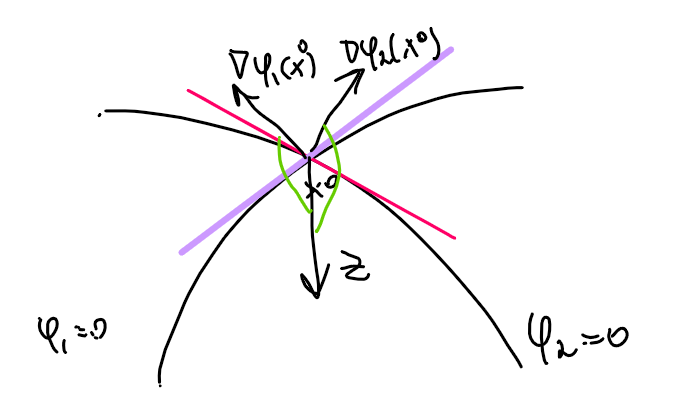
\includegraphics[width=0.25\textwidth]{2023-05-08 153256.png}
% \end{wrapfigure}

\begin{definition}
    Направление z называется прогрессивным в точке $x^0$, если
    \[\begin{cases}
        (\nabla \phi_i(x^0), z)<0 \quad \forall i \in I_0 \\
        (\nabla f(x^0), z)<0 
    \end{cases}\]
\end{definition}
\begin{remark}
    Если направление z прогрессивно, то сделав достаточно малый шаг h из $x^0$ вдоль z, получаем:
    $x^1 = x^0 + hz$, 
    \begin{enumerate}
        \item $x^1 \in D$
        \item $f(x^1) < f(x^0)$
    \end{enumerate}
\end{remark}

\subsection{Критерий оптимальности}
\begin{theorem}[Критерий оптимальности]
    $x^* \in D$ - оптимальное решение задачи ВП $\Leftrightarrow$
    в точке $x^*$ нет прогрессивного направления, т.е не существует $z\in R^n$: 
    \[\begin{cases}
        (\nabla \phi_i(x^0), z)<0 \quad \forall i \in I_0 \\
        (\nabla f(x^0), z)<0 
    \end{cases}\]
\end{theorem}
\begin{proof}
    \begin{lemma}
        пусть $f(x)$ выпукла на D и дифференцируема в точке $x^*\implies (\nabla f(x^*), x - x^*)\le\Delta f(x^*) = f(x) - f(x^*)$ 
    \end{lemma}
    \begin{proof}
        Пусть $z = x - x^*$.
        \[(\nabla f(x^*), z) = f_z'(x^*)=\lim_{\lambda \to 0+0} \frac{f(x^* +\lambda z) - f(x^*)}{\lambda} = \lim_{\lambda \to 0+0}\frac{f(x^* +\lambda (x-x^*)) - f(x^*)}{\lambda}=\]
        \[=\lim_{\lambda\to 0+0}\frac{f((1-\lambda)x^* +\lambda x) - f(x^*)}{\lambda} \le \lim_{\lambda \to 0+0} \frac{(1-\lambda) f(x^*)+\lambda f(x) - f(x^*)}{\lambda} = \lim_{\lambda \to 0+0}\frac{\lambda (f(x) - f(x^*))}{\lambda} = f(x) - f(x^*)\]
    \end{proof}
    $\Rightarrow$ От противного. Если в $x^* \exists$ прогрессивное направление, то в силу зам. 2, сделав достаточно малый шаг в направлении z, мы получим точку с меньшим значением целевой функции.
    
    $\Leftarrow$ Пусть в точке $x^*$ нет прогрессивного направления. Докажем, что $x^*$ оптимальное решение. 
    
    Предположим, что это не так и существует $x'\in D$ $f(x')< f(x^*)$

    В силу непрерывности функции $f(x)$ существует окрестность $O_{x'} : \forall x\in O_{x'}$ $f(x) < f(x^*)$

    Рассмотрим $(.) \bar{x}$ - точка Слейтера, т.е. $\forall \phi_i(\bar{x}) < 0 \forall i$ и рассмотрим $[x', \bar{x}]$
    
    Любая точка этого отрезка записывается как $x^\lambda = (1- \lambda)x' + \lambda \bar{x}\lambda \in (0,1)$

    Для некоторого $\lambda_0$ соответствует точка 
    \[x^{\lambda_0} = (1-\lambda_0)x' + \lambda_0\bar{x}\in O_{x'},\]
    т.е $f(x^{\lambda_0})< f(x^*)$

    Докажем, что $x^{\lambda_0}$ является внутренней точкой D.
    \[\forall i \phi_i(x^{\lambda_0}) = \phi_i((1-\lambda_0)x' + \lambda_0\bar{x})\le^{\text{выпуклость}} (1-\lambda_0)\phi_i(x')_{\le 0} + \lambda_0\phi_i(\bar{x})_{< 0} < 0\implies\]
    $x^{\lambda_0}$ внутренняя точка

    Пусть $z = x^{\lambda_0} - x^*$ 
    Докажем, что z - прогрессивное направление в $x^*$
    
    \[I_0 = \{i | \phi_i(x^*) = 0\}\]
    \[\forall i\in I_0 (\nabla \phi_i(x^*), z) = (\nabla \phi_i(x^*), x^{\lambda_0}-x^*)\le^{\text{лемма}} \phi_i(x^{\lambda_0} - \phi_i(x^*)) < 0 \implies\]
    z - возможное направление \[\leq (\nabla f(x^*), x^{\lambda_0} - x^*) \le^{\text{лемма}} f(x^{\lambda_0})_{<0} - f(x^*)_{\ge 0} < 0\implies\]
    z  - прогрессивное направление, противоречие
\end{proof}
    \subsection{Каноническая задача ВП}
    \begin{definition}
        Канонической задачей ВП называется задача ВП с линейной целевой функцией, т.е $f(x) = (c, x)\to \min$
    \end{definition}
    \paragraph*{Свойства}
    \begin{enumerate}
        \item $\nabla f = c = const$
        \item оптимальное значение функции достигается на границе
    \end{enumerate}

\begin{theorem}[эквивалентности]
    Для любой задачи ВП, $\exists$ эквивалентная ей каноническая ЗВП
\end{theorem}
Идея:
\[f(x) \to min \quad x_{n+1} \to \min\]
\[\phi_i(x)\le 0 , i = 1, \dots, m \quad f(x) - x_{n+1} \le 0, \phi_i(x)\le 0 , i = 1, \dots, m\]
\[x\in G = R^n \quad x\in G = R^{n+1}\]

\newpage
\subsection{Метод возможных направлений(модификация Зойтендейка)}
Рассмотрим каноническую задачу ВП (I)
\begin{center}
    \(f(x) = (c, x) \to \min\) \\
    \(\phi_i(x) \le 0, i = 1, \dots, m\)\\
    \(x \in R^n\)
\end{center}
$\phi_i - $выпуклая, непрерывно дифф.
Выполнено условие Слейтера, $x^0$- начальная допустимая точка $\in D$

Задаем начальный уровень допустимой близости к границе $\delta^0>0$

\[I_0 = \{i | \phi_i(x^0) = 0\}\]

\[I_\delta = \{i | -\delta^0<\phi_i(x^0) \leq 0\}\]
Выпишем одну итерацию алгоритма.
\begin{enumerate}
    \item[шаг 0] (проверка близости $x_0$ к границе D)

    Определяем для текущих $x^0, \delta^0$ множества $I_0, I_{\delta_0}$
    (безусловно активные и условно активные ограничения)
    
    [На практиках отрезок $-\delta^0 \le \phi(x^0) \le 0$]
    \item[шаг 1] Нахождение прогрессивного направления z в $x^0$

    Составляем вспомогательную задачу ЛП:
    \[y\to \min\]
    \[(\nabla \phi_i(x^0), z)\le y ,\forall i \in I_\delta\]
    \[(c, z)\le y, \textbf{может быть и не линейное ограничение actually}\]
    \[\textbf{тогда просто скалярное произведение градиента и z}\]
    \[|z_j|\le 1, j = 1, \dots, n - \text{условие нормировки, }\textbf{зам 1}\]
    \[y \le 0, \textbf{зам 2}\]
    Решаем задачу ЛП (она везде разрешима, \textbf{зам 3})

    [Замены $|z_j|\le 1\implies u_j = x_j - 1$, тем самым получаем неотрицательную переменную]

    Возможны следующие случаи.
    \begin{enumerate}
        \item \begin{enumerate}
            \item $y^0 = y^* < -\delta^0\implies z^0$ - прогрессивное направление и на следующей итерации полагаем $\delta^1 = \delta^0$
            \item $-\delta^0 \le y^0 < 0 \implies z^0$ - также прогрессивное, но на след итерации $\delta^1 = \delta^0/2$($\delta^0$ характеризует скорость убывания)
        \end{enumerate}
        Переходим на шаг 2
        \item Если $y^0 = y^* = 0, $ то строим аналогичную задачу ЛП, только индексы i из $I_0$. Если и в этом случае $y^* = 0$, то прогрессивного направления нет и текущая точка оптимальна, \textbf{СТОП}

        Если же $y^* < 0\implies$ соотв. z - прогрессивное направление и на след. итерацию $\delta^1 = \delta^0 /2$, шаг 2
    \end{enumerate}
    \item[шаг 2](Поиск величины шага в прогрессивном направлении)

    \[x^1 = x^0 + zh\]
    h надо найти, величина шага определяется как наименьший положительный корень уравнений $\phi_i(x^0 +zh) = 0, \forall i = 1, \dots, m$

    Далее выполняем шаг величины h в направлении z, $f(x^1) < f(x^0)$, т.к шаг делает в прогрессивном направлении $\implies x^1, \delta^1$ - вход для следующей итерации, переходим к ней.
\end{enumerate}
\paragraph*{Замечания}
\begin{enumerate}
    \item $|z_j|\le 1, j = 1, \dots, n.$ Без этого условия соответствующая задача ЛП неразрешима, z - прогрессивное направление, y - значение целевой функции. $\implies$ tz - прогрессивное направление 

    \[(\nabla \phi_i(x^0), tz) \le (ty), i\in I_s\]
    \[(\nabla f(x^0), tz) = ty\implies\] 
    ty - соотв. значение целевой функции.

    $ty\to -\infty$ при $t \to +\infty\implies$ функция неограничена на D.

    \item $y \le 0$ - зачем? для удобства получения канонической задачи ЛП. Можно так сделать, так как рассматриваем нулевое решение - которое является допустимым $(0, \overline{0})\implies y ^*\le 0$
    
    Наличие этого условия не влияет на оптимальное значение целевой функции.

    \item ВЗЛП является разрешимой, так как $D\neq \varnothing$ и целевая функция ограничена как непрерывная функция, заданная на замкнутом ограниченном множестве.

\end{enumerate}
\paragraph*{Поиск начального допустимого решения}

Пусть $\delta_0 > 0$ - произвольный начальный допустимый уровень.

Составляем вспомогательную задачу (она каноническая, t линейно):
\[t \to \min\]
\[\phi_i(x) - t \le 0, i = 1, \dots, m\]
\[x\in R^n\]
\[t\in R\]
\begin{itemize}
    \item[шаг 1] Берем $x^0$ - произвольный вектор, $t^0 = \max_{i = 1, \dots, m}\phi_i(x^0), (t^0, x^0)$ - допустимое решение.
    \item[шаг 2] Решаем задачу вспомог. с начальным решением $(t^0, x^0)$ до тех пор, пока $t^k\le 0\implies x^k$ - доп. решение исходной задачи. (такое $t^k$ в силу выполнения условия Слейтера)
\end{itemize}
\begin{theorem}[о сходимости метода возможных направлений]
    Рассмотрим каноническую задачу выпуклого программирования, в которой $\phi_i(x), i = 1, \dots, m$ являются непрерывными и дифференцируемы, выполнено УС, D - ограничена.

    Если есть некая последовательность точек $\{x^k\}_{k = 1}^\infty$, получаемых методом возможных направлений (МВН), тогда
    \begin{enumerate}
        \item $\{f(x^k)\}_{k = 1}^\infty \to f^*$
        \item Любая предельная точка $\{x^k\}_{k = 1}^\infty$ является оптимальным решением ЗВП.
    \end{enumerate} 
\end{theorem}
\begin{proof}
    Без доказательства.
\end{proof}
\subsection{Теорема Куна-Таккера о седловой точке}
Рассмотрим задачу выпуклого программирования следующего вида:
\[f\to \min\]
\[\phi_i(x)\le 0, i = 1, \dots, m\]
\[x \in G \subseteq \mathbb{R}^n\]
$f, \phi_i$ - выпуклые в множестве G, G - выпуклое и замкнутое. Выполнено УС.

Для этой задачи определим функцию Лагранжа
\[L(x, y) = f(x) +\sum_{i = 1}^m y_i \phi_i(x), \text{где } y_i\ge 0, i = 1, \dots, m, \text{ в отличие от классического метода множителей Лагранжа}\]
\begin{definition}
    $(x^*, y^*)$, где $x^*\in G, y^*\ge \overline{0}$, называется седловой точкой функции Лагранжа, если 
    \[L(x^*, y)\le L(x^*, y^*)\le L(x, y^*), \forall x\in G, \forall y\ge 0 \]
\end{definition}
\begin{theorem}[Теорема Куна-Таккера о седловой точке]
    $x^*\in G$ - оптимальное решение задачи выпуклого программирования тогда и только тогда, когда существует $y^* \ge 0$, такое что $(x^*, y^*)$ является седловой точкой функции Лагранжа    
\end{theorem}
\begin{proof}
    При доказательстве используем следующее утверждение
    \begin{theorem}[Теорема Фaна(ударение на первую а)]
        Пусть G -  выпуклое, замкнутое множество в $R^n, g_i, i = 0, \dots, m$ - выпуклые функции на G. 
        Предположим, что система 
        \[\begin{cases}
            g_0(x)< 0\\
            g_i(x) \le 0, i = 1, \dots, m
        \end{cases}\]
        не имеет решений, тогда существует такой вектор c:  ($\left\lVert c\right\rVert  = 1, c_j \ge 0, i = 0, \dots, n$) такой, что 
        \[\sum_{i = 0}^m c_i g_i(x)\ge 0, \forall x\in G\]
    \end{theorem}
    $\implies$ Пусть $x^* \in G$ - опт. решение ЗВП.$\implies \forall x\in G f(x) \ge f(x^*)$

    Докажем, что $\exists y^* \ge 0 : (x^*, y^*)$ - седловая точка функции Лагранжа

    \[\begin{cases}
        f(x)- f(x^*)< 0 \\ 
        \phi_i(x) \le 0, i = 1, \dots, m \\
    \end{cases}\]
    несовместная система

    Тогда по теореме Фана существует с ($\left\lVert c\right\rVert  = 1, c_i \ge 0$)
    \[c_0(f(x) - f(x^*)) + \sum_{i = 1}^m c_i \phi_i(x)\ge 0, \forall x\in G\]
    
    \begin{enumerate}
        \item $c_0> 0$

        $c_0$ не может быть равным нулю, подставляем точку Слейтера неравенство не выполняется (одно слагаемое 0, другое строго меньше 0 (из УС)).

        Значит, можно делить на $c_0$
        \item Разделим неравенство на $c_0$, назовем $y_i^* = \frac{c_i}{c_0}\ge 0$
        \[(f(x) - f(x^*)) + \sum_{i = 1}^m y_i^* \phi_i(x)\ge 0, \forall x\in G\]
        \item Докажем, что 
        \[\sum_{i = 1}^m y_i^* \phi_i(x^*) = 0\]
        (типа условие дополняющей нежесткости)

        Подставим в последнее полученное большое неравенство $x = x^*$
        \[\sum_{i = 1}^m y_i^* \phi_i(x^*)\ge 0\]

        Но при $x = x^*$ $\phi_i(x^*)\le 0, y_i^*\ge 0\implies$
        \[ \sum_{i = 1}^m y_i^* \phi_i(x^*)\le 0\]
        Доказано.
        \item $L(x^*, y)\le L(x^*, y^*)\le L(x, y^*)$

        $L(x^*, y) = f(x^*) +\sum_{i = }^{m} y_i \phi_i(x^*)\le f(x^*) = f(x^*) + \sum_{i = 1}^m y_i^* \phi_i(x^*)$ Левое неравенство доказано.

        Давайте правое.

        (как идет так идет................)

        $L(x^*, y^*) = f(x^*) +\sum_{i = 1}^{m}y_i^* \phi_i(x^*)\le f(x) +\sum_{i =1 }^{m} y_i^* \phi_i(x) - L(x, y^*)$
        доказано.


    \end{enumerate}        
    В другую сторону:

    $x^* \in G, y^* \ge 0: (x^*, y^*)$ - седловая точка

    Доказать, что $x^*$ - оптимальное решение ЗВП.

    $x^*\in G, y^* \ge 0$ образуют седловую точку функции функции Лагранжа \[L(x^*, y)\le^{(*)} L(x^*, y^*)\le^(**) L(x, y^*) \forall x\in G, \forall y \ge0\]

    Доказать, что $x^*$ - опт решение (I) 
    
    Докажем, что $x^* \in G$, т.е $\phi_i(x^*)\le 0 \forall i = 1\dots m$

    От противного $\exists k \phi_k(x^*)>0$

    Применим  (*)  для y = (0, \dots, t, 0\dots), t >0, t на k-атом месте

    \[f(x^*) + t \phi_k(x^*) \le f(x^*)+\sum_{i = 1}^m y_i^* \phi_i(x^*)\]
    $f(x^*)$ - сократится 

    \[t\phi_k(x^*) \le \sum_{i = 1}^m y_i^* \phi_i(x^*)\]
    $\phi_k(x^*)>0$ при t стремящемся к бесконечности стремится к бесконечности, а сумма является константой - получаем противоречие

    $\implies \phi_i(x^*)\le 0 \; \forall i = 1, \dots, m\implies x^* \in D$

    Докажем, что $\sum_{i = 1}^m y_i^* \phi_i(x^*) = 0$
    
    Подставим в (*) y =0, $f(x^*)\le f(x^*) + \sum_{i = 1}^m y_i^* \phi_i(x^*) \implies \sum_{i = 1}^m y_i^* \phi_i(x^*) \ge 0$
    
    но \[\phi_i(x^*)\le 0 , \forall i, y^*_i\ge0 \implies \sum_{i = 1}^m y_i^* \phi_i(x^*) \le 0 \implies \sum_{i = 1}^m y_i^* \phi_i(x^*) = 0\]
    
    Докажем, что для любого x из D $f(x)\ge f(x^*)$

    Рассмотрим (**)

    \[f(x^*) + \sum_{i = 1}^m y_i^* \phi_i(x^*) \le f(x) + \sum_{i = 1}^m y_i^* \phi_i(x)\]
    \[y^*_i \ge0, \phi_i(x)\le 0\implies \sum_{i = 1}^m y_i^* \phi_i(x)\le 0 \implies\]
    \[f(x^*)\le f(x)\implies x^* - \textbf{оптимальное}\]
\end{proof}
\subsection{Теорема Куна-Таккера в дифференциальной форме}
\subsubsection{Дифференциальная форма 1}
Рассмотрим задачу ВП  (I)
\[f(x)\to \min\]
\[\phi_i(x)\le 0, i = 1, ..., m\]
\[x_j \ge 0, j = 1, ..., n\]
\[G = \{x\in R^n, x_j \ge 0, j = 1, ..., n\}\]
$f, \phi_i$ - непрерывно дифференцируемые на G

Выполнено УС

\[L(x, y) = f(x) +\sum_{i = 1}^{m}y_i \phi_i(x), y_i\ge 0 , i = 1, \dots, m\]
Обозначим \[\nabla_x L(x^*, y^*) = (\frac{\partial L}{\partial x_1}, ..., \frac{\partial L}{\partial x_n})|_{(x^*, y^*)}\]

\[\nabla_y L(x^*, y^*) = (\frac{\partial L}{\partial y_1}, ..., \frac{\partial L}{\partial y_m})|_{(x^*, y^*)} = (\phi_1(x^*), \dots, \phi_m(x^*))\]
\begin{theorem}[Куна-Таккера в дифференциальной форме 1]
    Точка $x^* \ge 0$ является оптимальным решением задачи (I) тогда  и только тогда, когда существует $y^*\ge 0$ такой, что выполняются следующие условия:
    \begin{enumerate}
        \item $\nabla_x L(x^*, y^*) \ge 0,$ т.е. $\frac{\partial L(x, y^*)}{\partial x_j} |_{x = x^*} \ge 0, \forall j = 1, \dots, n$
        \item $(x^*, \nabla_x L(x^*, y^*)) = 0$ т.е $\sum_{i = 1}^n x^*_j\frac{\partial L(x, y^*)}{\partial x_j}|_{x^*} = 0$
        \item $\nabla_y L(x^*, y^*) \le 0,$ т.е $\phi_i(x^*)\le 0, i = 1, ..., m$
        \item $(y^*, \nabla_y L(x^*, y^*)) = 0, $ т.е $\sum_{i = 1}^{m}y^*_i \phi_i(x^*) = 0$
    \end{enumerate}
\end{theorem}
\begin{proof}
    Докажем слева направо 

    $x^*\ge 0$ - оптимальное решение. По теореме Куна Таккера существует $y^*\ge 0$
    \[L(x^*, y) \le L(x^*, y^*)\le L(x, y^*), \forall x\ge0, \forall y \le 0\]
    Для каждого $j = 1, \dots, n$ рассмотрим точку $x^j = (x_1^*,\dots, x_{j-1}^*, x_j^*, \dots, x_n^*)$. Из (**) следует, $x^j$ - глобальный минимум функции $L(x^j, y^*)$ - функция от одной переменной на множестве $ \{x_j\in R: x_j \ge 0\}$
    
    Условия 1), 2) теоремы - необходимые условия локального минимума на неотрицательной полуоси

    $x_j^* > 0, \frac{\partial L}{\partial x_j}|_{(x^*, y^*)}$

    $x_j^* = 0 \frac{\partial L}{\partial x_j}|_{(x^*, y^*)} \ge 0 $

    По аналогии из (*) получаются неравенства 3), 4) теоремы как необходимые условия локального максимума

    Справа налево: Пусть выполняются условия 1)-4) для некоторого $x^*\ge 0, y^*\ge 0$

    Докажем, что $(x^*, y^*)$ - седловая точка функции Лагранжа
    
    При фиксированном $y^*\ge 0 $ функция Лагранжа

    \[L(x, y^*) = f(x) + \sum_{i = 1}^m y_i^* \phi_i(x)\] - выпуклая функция

    По лемме о приращении и градиенте для выпуклой функции 

    \[\forall x\ge0, L(x, y^*) - L(x^*, y^*)\ge (\nabla_x L(x^*, y^*), x-x^*) = (\nabla_x L(x^*, y^*), x) - (\nabla_x L(x^*, y^*), x^*)\]\

    \[(\nabla_x L(x^*, y^*), x^*) = 0\] по 2 условию из Теоремы
    
    \[(\nabla_x L(x^*, y^*)\ge0, \text{по 1}, x\ge 0)\]
    \[(\nabla_x L(x^*, y^*), x) - (\nabla_x L(x^*, y^*), x^*) \ge 0\]
    доказали (**)

    \[L(x^*,  y) - L(x^*, y^*) = f(x^*) +\sum_{i=1}^{m}y_i \phi_i(x^*) - f(x^*) - \sum_{i= 1}^m y_i^* \phi_i(x^*) \le 0 \implies\]
    вып (*)

    [Применили 3 и 4 для для слагаемых-сумм, последняя сумма равна 0, а у предпоследней $y_i\ge0, \phi_i\le 0$]
\end{proof}
\subsubsection{Дифференциальная форма 2}
Рассмотрим задачу ВП (II)
\[f(x)\to \min\]
\[\phi_i(x)\le 0, i = 1, ..., m\]
\[x\in R^n\]
\[G = R^n\]
$f, \phi_i$ - непрерывно дифференцируемые на G

Выполнено УС

\begin{theorem}[Куна-Таккера в дифференциальной форме 2]
    Точка $x^*\in R^n$ является оптимальной точкой задачи (II)
    тогда и только тогда, когда существует $y^*\ge 0$ такое, что выполняются условия
    \begin{enumerate}
        \item $\nabla_x L(x^*, y^*) = 0,$ т.е.
        $\frac{\partial L(x, y^*)}{\partial x_j} |_{x = x^*} = 0, \forall j = 1, \dots, n$
        \item $\nabla_y L(x^*, y^*) \le 0,$ т.е $\phi_i(x^*)\le 0, i = 1, ..., m$
        \item $(y^*, \nabla_y L(x^*, y^*)) = 0, $ т.е $\sum_{i = 1}^{m}y^*_i \phi_i(x^*) = 0$, или $\forall i: y^*_i \phi_i(x^*) = 0$
    \end{enumerate}
\end{theorem}
\begin{proof}
    самостоятельно
\end{proof}
\section{Квадратичное программирование}
\subsection{Квадратичная функция}
\begin{definition}[Квадратичная форма]
    Квадратичной формой от n переменных называется функция вида
    \[g(x)  = (cx, x) = \sum_{i=1}^{n}\sum_{j=1}^{n}c_{ij}x_i x_j\], где C - симметричная матрица, $c_{ij} = c_{ji}$

    Диагональные элементы - коэффициенты при квадратах переменных, а остальные - половине коэффициентов
\end{definition}
\begin{example}
    \[g(x_1, x_2) = 3x_1^2 -3x_1x_2 + 4x_2^2, C =\begin{pmatrix}
        3 & -\frac32\\
        -\frac32 & 4
        \end{pmatrix}\]
    
\end{example}
\begin{definition}
    Квадратичная форма называется неотрицательно определенной, если $\{\forall x\in R^n  | x\neq 0\}$ выполняется $g(x)\ge 0$, и положительно определенной если $\{\forall x\in R^n  | x\neq 0\}$ выполняется $g(x) > 0$
\end{definition}
\subparagraph*{Способы проверки неотрицательной/положительной определенности}
\begin{enumerate}
    \item Критерий Сильвестра

    Квадратичная форма является положительно определенной, если ее главные миноры положительны, и неотрицательно определенной, если ее главные миноры неотрицательны
    \item Через собственные числа

    \begin{enumerate}
        \item Квадратичная форма $(Cx, x)$ положительно определена, если корни характеристического многочлена ($|C-\lambda E| = 0$) положительны, и неотрицательно определена, если корни характеристического многочлена неотрицательны, и хотя бы 1 корень равен 0.
    \end{enumerate}
\end{enumerate}
\begin{definition}[Квадратичная функция]
    Функция вида $f(x) = \sum_{i = 1}^n \sum _{j = 1}^nc_{ij}x_i x_j +\sum_{i = 1}^n p_i x + p_0 = (Cx, x) + (p, x) + p_0, p \in R^n, p_0\in R$ 
\end{definition}
\begin{theorem}
    Квадратичная функция f(x) выпукла тогда и только тогда, когда квадратичная форма $(Cx, x)$ неотрицательно определена
\end{theorem}
\begin{proof}
    Так как \[(p, x)+ p_0\] не нарушает выпуклости, будем доказывать только для нелинейной части, т.е для g(x) = (Cx, x).
    \begin{lemma}
        Для любых $x^1, x^2 \forall \lambda \in (0, 1)$
        \[(1 - \lambda)g(x^1) + \lambda g(x^2) - g((1-\lambda)x^1 + \lambda x^2 ) = \lambda (1 - \lambda ) g(x^1 -x^2)\]
        \[(1 - \lambda)(Cx^1, x^1) + \lambda(Cx^2, x^2) - (C ((1-\lambda)x^1 + \lambda x^2 ), (1-\lambda)x^1 + \lambda x^2 )=\]
        \[=(1 - \lambda)(Cx^1, x^1) + \lambda(Cx^2, x^2) -(1-\lambda)^2 (Cx^1, x^1) - (1 - \lambda)\lambda (Cx^1, x^2)- \lambda (1-\lambda)(Cx^2, x^1) - \lambda ^2 (Cx^2, x^2)= \]
            \[= (1 - \lambda )(\lambda )(Cx^1, x^1) - \lambda (1- \lambda )(Cx^2, x^2)+\lambda (1 - \lambda)(Cx^2, x^1) - \lambda (1- \lambda)(Cx^1, x^2) = \]
            \[\lambda (1-\lambda)((Cx^1, x^1 - x^2) - C(x^2, x^1 - x^2)) = \lambda(1- \lambda) g(x^1 - x^2)\]
    \end{lemma}
    $\Rightarrow$ Если функция g(x) выпукла, то левая часть 
    $\lambda(1-\lambda) g(x^1 - x^2)\ge 0\implies g(x^1 - x^2) \ge 0$
    для любых $x^1, x^2$

    Любой вектор $x\in R^n$ можно представить как разность $x^1, x^2 \implies$ неопределенно определена

    $\Leftarrow$ С неотрицательно определена, аналогично $\lambda (1-\lambda)g(x^1- x^2)\ge 0 \implies$ левая часть выражения в лемме больше, либо равна 0$\implies g(x) выпукла$
\end{proof}
\subsection{Задача квадратичного программирования}
\begin{definition}
    Задача $f(x) = \sum_{i=1}^{n}\sum_{j=1}^{n} c_{ij}x_i x_j +\sum_{j  = 1}^{n}p_j x_j +p_0\to \min$
    \[\sum_{j = 1}^n a_{ij}x_j \le b_i, i = 1, \dots, m\]
    \[x_j\ge 0, j = 1, \dots, n\]
    называется задачей квадратичного программирования
\end{definition}
В матричном виде
\[f(x) = (Cx, x) + (p, x) +p_0\]
\[Ax \le b\]
\[x \ge 0\]
\begin{remark}[1]
    Далее $p_0 = 0$
\end{remark}
\begin{remark}[2]
    $c\ge 0$ задача кв. программирования является задачей выпуклого программирования, верна теорема Куна-Таккера (в дифференциальной форме 1, так как x из $\mathbb{R}^n_+$)
\end{remark}
\begin{theorem}
    Вектор $x^*\ge 0$ является оптимальным решением задачи КП $\Leftrightarrow \; \exists$ неотрицательные векторы $y^*, u^*\in R^m$и $v^*\in R^n$ что выполняется 
    \begin{enumerate}
        \item $2Cx^* + A^T y^* - v^* = -p$
        \item $Ax^* + u^* = b$
        \item $(x^*, v^*) = 0$
        \item $(y^*, u^*) = 0$
    \end{enumerate}  
\end{theorem}
\begin{proof}
    Рассмотрим задачу КП как задачу ВП
    \[f = (Cx, x) + (p, x)\to \min\]
    \[Ax - b\le 0\]
    \[x\ge 0\]
    \[L(x, y) = (Cx, x) + (p, x) + (y, Ax -b )\forall y\ge 0 , \forall x\ge 0\] - функция Лагранжа

    Используем теорему Куна-Таккера в диф. форме 1:
    
    Точка $x^* \ge 0$ является оптимальным решением задачи (I) тогда  и только тогда, когда существует $y^*\ge 0$ такой, что выполняются следующие условия:
    \begin{enumerate}
        \item $\nabla_x L(x^*, y^*) \ge 0,$ т.е. $\frac{\partial L(x, y^*)}{\partial x_j} |_{x = x^*} \ge 0, \forall j = 1, \dots, n$
        \item $(x^*, \nabla_x L(x^*, y^*)) = 0$ т.е $\sum_{i = 1}^n x^*_j\frac{\partial L(x, y^*)}{\partial x_j}|_{x^*} = 0$
        \item $\nabla_y L(x^*, y^*) \le 0,$ т.е $\phi_i(x^*)\le 0, i = 1, ..., m$
        \item $(y^*, \nabla_y L(x^*, y^*)) = 0, $ т.е $\sum_{i = 1}^{m}y^*_i \phi_i(x^*) = 0$
    \end{enumerate}
    $\implies$ применим условия 1 и 3 к нашей задаче и приведем их к равенствам 
    \begin{enumerate}
        \item $2Cx^* + A^T y^* - v^* = -p$
        \item $Ax^* u^* = b$
    \end{enumerate}
    Применим условие 2 и 4 к нашей задаче

    $\nabla_x L(x, y)|_{(x^*, y^*)} = 2Cx^* + A^T y^* + p = v^*$

    $2) (x^*, v^*) = 0$

    $\nabla_y L(x, y)|_{(x^*, y^*)} = Ax^* - b = -u^*$

    $4) (y^*, -u^*) = 0\implies (y^*, u^*) = 0$

    Условие теоремы эквивалентно условиям теоремы Куна-Таккера
\end{proof}
Вывод: для решения задачи квадратичного программирования достаточно найти неотрицательные векторы $x^*, y^*, u^*, v^*:$

\begin{enumerate}
    \item $2Cx^* + A^T y^* - v^* = -p$
    \item $Ax^* + u^* = b$
    \item $(x^*, v^*) = 0$, т.е $x_j^* v_j^* = 0\; \forall j = 1, \dots, n$
    \item $(y^*, u^*) = 0$ т.е $y_i^* u_i^* = 0\; \forall i = 1, \dots, m$
\end{enumerate}  
\begin{remark}
    \begin{enumerate}
        \item 1, 2 - СЛУ n+m уравнений, 2n+2m переменных
    \end{enumerate}
\end{remark}
\begin{theorem}
    Если $\exists$ неотрицательное решение системы 1-2, уд. 3-4, то существует и базисное неотрицательное решение этой же системы, удовлетворяющее тем же свойствам
\end{theorem}
\begin{proof}

\end{proof}
\subsection{О методах решения задач квадратичного программирования}
Все методы основаны на методах решения системы 1 - 4 

\begin{enumerate}
    \item метод Баранкина-Дорфмана
    \item Франка-Вулфа
    \item метод Вулфа
\end{enumerate}
в 1-2 с помощью некоторого базиса строится некоторое базисное решение 1-2, которое не обязательно удовлетворяет 3-4, а затем с помощью вспомогательных симплексных преобразований добиваются выполнения условий 3-4,

а в 3 с помощью введения искусственных переменных строится вспомогательная ЗЛП, которая решается симплекс методом, при этом начальное базисное решение удовлетворяет 3-4, и далее решаем эту задачу, следя за выполнением 3-4 на каждой итерации (если C положительно определена, то метод сходится)
\end{document}